\documentclass{article}
\usepackage[utf8]{inputenc}
\usepackage{graphicx}
\usepackage{hyperref}
\graphicspath{ {images/} }
\usepackage[a4paper]{geometry}
\geometry{verbose,tmargin=2cm,bmargin=2cm,lmargin=2cm,rmargin=2cm}
\title{BET overovani bezpecnosti}
\author{opltfrantisek }
\date{October 2017}

\usepackage{natbib}
\usepackage{graphicx}

\begin{document}

\maketitle
\tableofcontents
\section{Bezpečnost IT}
Zabezpečováním IT se označuje proces dosažení a udržení důvěrnosti, integrity, dostupnosti,
prokazatelnosti, odpovědnosti, autenticity a spolehlivosti informací a služeb IT na takové úrovni, aby
případné náklady na narušení bezpečnosti převyšovaly náklady na její dosažení. Bezpečnost IT v organizaci
závisí především na přístupu managementu organizace a tato by měla být nedílnou součástí
bezpečnostní politiky organizace
\subsection{Problémy bezpečnosti IT}
 Sále u nás najdete firmy,
pro které jsou jejich informace otázkou existence, ale přesto příslovečně nehnuly v bezpečnosti
prstem a patří mezi ty, jež spoléhají na štěstí.
A pak jsou firmy, které se pro svůj úspěch snaží udělat více, a bezpečnost řeší nebo řešit začaly.
Management těchto firem provedl v určitém stádiu důležitý "mentální krok" (ještě ne vlastní krok ře-
šení, spíše příprava na odraz).
Co obnáší "mentální krok"? Management se rozhodl informační bezpečností skutečně zabývat,
což obnáší všechny, nebo alespoň některé následující rysy:
\begin{itemize}
    \item vyčlenění interních lidských zdrojů (zřízení útvaru bezpečnosti, jmenování bezpečnostního
manažera, alokace pracovníků jiných útvarů)
    \item vyhrazení finančních prostředků
    \item ochota spolupracovat na řešení bezpečnosti s externími dodavateli
    \item připravenost vzít na sebe zodpovědnost za bezpečnost na nejvyšší úrovni
    \item uvědomění si potřeby spustit systematický proces řešení
    \item smíření se s faktem, že řešení bezpečnosti znamená věnovat se této oblasti natrvalo
\end{itemize}
Důvodů, proč se management pohnul, může být několik - prožité bezpečnostní incidenty,
závěry auditu, rozhodnutí majitelů, snaha získat konkurenční
výhodu, srovnání obdobných firem v oboru atd. Podstatné je, že toto rozhodnutí bývá jen výjimečně
podloženo tvrdými fakty typu návratnosti investic (ROI). Proto bývá toto rozhodnutí těžké
a "mentální krok" s sebou přináší chápání investic do bezpečnosti analogicky jako nákladů spojených
s pojištěním.
\subsection{Řešení problémů bezpečnosti IT}
\subsubsection{Strategie informační bezpečnosti}
tomto kroku je potřeba udělat dva hlavní kroky: \newline
• definovat hlavní cíle v oblasti informační bezpečnosti (co a jak chránit)\newline
• navrhnout a schválit parametry dalších kroků, ideálně ve formě projektu/ů\newline
První krok vlastně představuje zhmotnění "mentálního kroku". Management stanovuje priority
řešení a ty se musí promítnout do cílů a parametrů. Typickými výstupy této části bývá definiční
projektová dokumentace a ideálně také Celková bezpečnostní politika - stručný dokument deklarující
podporu managementu v oblasti bezpečnosti (nejen informační).
\subsubsection{Analýza rizik}
Analýza rizik musí poskytnout odpovědi na tři základní otázky:\newline
• Co se stane, když nebudou informace chráněny?\newline
• Jak může být porušena bezpečnost informací?\newline
• S jakou pravděpodobností se to stane?\newline
Existuje řada specializovaných metodologií na provádění analýzy rizik (např. FRAP, IRIS,
CRAMM) a tento krok typicky vyžaduje spolupráci s externími experty. Standardním výstupem analýzy
rizik je zpráva se sumarizací a prioritizací rizik plus návrh doporučených opatření na jejich eliminaci
nebo alespoň snížení.
\subsubsection{Informační bezpečnostní politika}
Analýza rizik provedená v předchozím kroku vede k detailnímu poznání organizace, jejích problé-
mů a potřeb. To umožňuje vytvořit klíčový bezpečnostní dokument - bezpečnostní politiku - a zohlednit
v něm specifika dané organizace. Jedná se o dokument, který je po přijetí managementem zá-
vazný pro celou společnost a který definuje východiska pro všechny další aktivity společnosti v oblasti
informační bezpečnosti. Hlavním cílem informační bezpečnostní politiky je:\newline
• definovat hlavní cíle při ochraně informací \newline
• stanovit způsob, jak bezpečnost řešit \newline
• určit pravomoci a zodpovědnosti \newline
\subsubsection{ Bezpečnostní směrnice a standardy}
Bezpečnostní politika definuje hlavní pravidla a zásady bezpečnosti. Ty je potřeba ještě dále
konkretizovat do podoby detailních pravidel a postupů - bezpečnostních směrnic a standardů.
Směrnice a standardy jsou součástí interní legislativy a jako takové se stávají závaznými pro organizaci.
\subsubsection{ Implementace bezpečnosti}
Zásady a pravidla politiky, resp. standardů a směrnic, se nenaplní automaticky jejich vytvořením
a přijetím. Je potřeba nastartovat aktivity (projekty), které bezpečnostní zásady uvedou do života.
Z tohoto pohledu se nejedná o uzavřený krok, ale spíše moment, kdy jsou zahajovány jednotlivé bezpečnostní
projekty, koordinované ustaveným bezpečnostním managementem. Příklady bezpečnostních\newline
projektů mohou zahrnovat:\newline
• bezpečnostní vzdělávání\newline
• havarijní plánování\newline
• zabezpečení připojení na internet\newline
• implementace infrastruktury veřejných klíčů\newline
\subsubsection{Monitorování a kontrola}
Pokud je ustaven bezpečnostní management a jsou schváleny klíčové bezpečnostní dokumenty, je
nutné zajistit dodržovaní definovaných pravidel a zásad a ovšem také zpětnou vazbu, která zajistí,
že se významné změny promítnou do příslušné dokumentace a do procesu řízení bezpečnosti.
Reakce na nově se objevující rizika, změny priorit organizace a změny okolního prostředí mohou vyvolat
potřebu vrátit se k některému z předchozích kroků řešení bezpečnosti a provést například doplňkovou
analýzu rizik, či doplnění chybějících bezpečnostních standardů a směrnic. 
\section{ověřování bezpečnosti}
\subsection{Proč se to dělá}Aby se zjistili případné zranitelnosti, které by mohl útočník využít. A tím i minimalizovali případné škody, které by mohl útočník napáchat. Najčastěji vznikají škody typu:
\begin{itemize}  
\item nedostupnost služby – služba není schopna obsluhovat legitimní uživatele (DoS,
DDoS útoky)
\item neoprávněný přístup útočníka k systému (počítač, server, databáze), kde může číst
či modifikovat data, měnit konfigurace
\item získání důvěrných informací – získání přihlašovacích údajů, adres, informací o financích
apod \ldots 
\end{itemize}

\subsection{Hledání slabých míst}
Pokud jsou nalezena nějaká slabá místa, může se naskytnout mož-
nost pro napadení systému. Dnešní nástroje pro odhalování zranitelností pracují po zadání
vstupních údajů a provedením požadovaného nastavení většinou automaticky. Výčet typických
činností těchto nástrojů:
\begin{itemize}  
\item procházení otevřených portů a služeb v celém bloku IP adres
\item zjištění typu operačního systému a aplikací, jejich verze, nainstalované záplaty
\item  zjištění nastavení, zabezpečení, autentizace aplikací nebo služeb
\item některé dovedou i nízkoúrovňové hádání hesel hrubou silou,
\item poskytnutí informací o možném řešení problému \ldots 
\end{itemize}
Výsledky testů odhalují základní bezpečnostní nedostatky systému a na testující osobě
spočívá úkol vyhodnotit, které problémy představují riziko v kontextu testovaného prostředí.
Může se stát, že nebezpečné chyby, označené automatickým softwarem, nemusí
v daném prostředí představovat vážné reálné riziko. Naopak malá detekovaná chyba může
vést k většímu útoku.
\subsection{Druhy testů}
\begin{itemize}  
\item Externí testy – jsou prováděny z vnější strany testované sítě a představují vnější hrozby
(např. útok hackera z internetu)
\item Interní testy – jsou prováděny z vnitřní strany testované sítě, které napodobují potencionálního
útočníka, který získal nějakým způsobem přístup do vnitřní sítě, nebo také
neloajálního zaměstnance
\end{itemize}
Podle úrovně znalostí o systému
\begin{itemize}  
\item Black-box testy – na testovaný systém se pohlíží jako na tzv. černou skříňku, kde jsou
známy pouze jeho vstupy a potencionální výstupy. Není známa vnitřní struktura systému.
Tato metoda je typická pro hackery, kteří mají jen běžnou veřejnou informaci (např. doménové
jméno serveru), kterou podrobuje dalšímu průzkumu.
\item White-box testy – na rozdíl od black-box testů jsou k dispozici všechny možné znalosti
o systému. V případě počítačové sítě, je to například topologie sítě, přítomná zařízení,
různé přístupové údaje, nastavení prvků atd. V případě testování aplikací se analyzují
zdrojové kódy a hledají se v něm chyby. Detailní informace o systému mohou umožnit
odhalení případných nedostatků v kratší době a celkově komplexnější analýzu systému.
\item Grey-box testy – kombinace předchozích dvou typů testů. Tester má pouze základní
znalosti o systému, které se snaží maximálně využít. Samotný test však probíhá z hlediska
potencionálního útočníka nebo v případě testování aplikace z hlediska uživatele.
\end{itemize}
Podle způsobu provedení
\begin{itemize}  
\item Manuální testy – tester je vykonává manuálně, umožňuje vytvořit testy na míru pro specifické
podmínky. Nevýhodou je, že jsou potřeba rozsáhlé znalosti testované oblasti a dovednosti
vytvořit testovací proceduru. Další nevýhodou je časová náročnost.
\item Automatizované testy – nástroje pro automatické testování vytvářejí profesionálové
v oboru a testerovi se stačí naučit s nástrojem pracovat a porozumět interpretaci vý-
sledků. Výhodou je rychlost aplikace testu, nevýhodou může být nemožnost otestovat
některé typy zranitelných míst.
\item Semiautomatizované testy – kombinace automatických a manuálních testů, snažící se
využít výhody obou způsobů.
\end{itemize}
\subsection{Metodologie testování}
\subsubsection{Plánování}
V této začáteční fázi je potřeba projednat a stanovit všechny organizační záležitosti. Pří-
prava a podepsání bezpečné smlouvy, sestavení týmu a vytvoření časového plánu.
Určují se detailní cíle, na které budou zaměřeny penetrační testy. Cíle penetračního
testování mohou být vymezeny například jen na webové aplikace, bezdrátové sítě, databáze
apod. Důležité je vymezit prioritní cíle, jelikož není vždy možné odhalit všechna zranitelná
místa. Záleží na přidělených prostředcích (finance, personál, čas), schopnostech testera, a
proto je potřeba se primárně zaměřit na místa a chyby, které představují pro firmu největší
riziko.
\subsubsection{ Sběr informací}
V další fázi nastává zjišťování co nejvíce informací o cílové síti. Používají se pojmy jako
information gathering nebo data mining. Získané informace se použijí jako vstup k další
fázi testování. Nejčastěji se jedná o základní informace jako rozsahy IP adres, jmenné
servery, kontaktní osoby, otevřené porty, síťové služby a jejich verze, operační systémy
síťových prvků. Takové informace je možné získat kombinací zdrojů jako whois a nástrojů
určených pro skenování portů. Další technikou v této fázi může být testování pravidel firewallu. K těmto účelům jsou dostupné automatizované nástroje.
\subsubsection{ Odhalování zranitelností}
Po získání informací z předchozí fáze nastává odhalování zranitelností. Za otevřenými
porty se skrývají nějaké síťové služby a operační systémy, na kterých běží, a ty mohou
představovat riziko. Při hledání chyb dojde k porovnávání jednotlivých verzí síťových slu-
žeb a operačních systémů s databází známých chyb. Také probíhají kontroly určitých chybných
konfigurací (misconfigurations). Výsledkem je seznam stanic či služeb, které obsahují
zranitelnosti nebo představují riziko. Nejčastěji se pro tento účel používají specializované
nástroje, které pracují automaticky.
\subsubsection{Zneužití chyb}
Tato fáze je samotné zneužívání nalezených zranitelností, tj. pokusy o prolomení bezpeč-
nostních mechanizmů. Exploitace je postavena na využívání nedostatků a chyb v aplikacích
a systémech. Časem se může objevit problém a neprolomitelný mechanizmus nemusí být
neprolomitelný navždy. Pro nejrůznější síťové služby existuje řada exploitů.
Po úspěšné exploitaci jedné služby se může otevřít cesta k další službě, která byla před
tím nepřístupná. Pak je třeba se vrátit ke sběru dat a hledání zranitelností pro nový cíl
\subsubsection{Konečná fáze}Konečná fáze zahrnuje shrnutí a předání výsledků penetračních testů. Cílem je prezentovat
zákazníkovi kvalitní závěrečnou zprávu, která povede ke zlepšení bezpečnosti firmy. Jedná-
li se o testování firemní sítě, výsledky by měly být prezentovány a prodiskutovány s IT
oddělením a vedením firmy
\subsection{Black box}
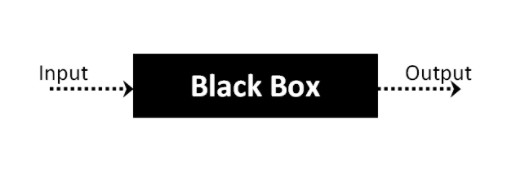
\includegraphics{bb}
Black box testování je realizováno bez znalosti vnitřní datové a programové struktury.
To znamená, že tester nemá k dispozici žádnou dokumentaci, binární ani zdrojové kódy. Tento způsob testování vyžaduje testovací scénáře, které jsou buď poskytnuty testerovi nebo si je tester u některých typů testů sám vytváří. Vzhledem k tomu, že jsou obvykle definovány typy a rozsahy hodnot přípustných a nepřípustných pro danou aplikaci a tester ví, jaký zadal vstup, tak ví i jaký výstup nebo chování může od aplikace očekávat. Black box testy mohou stejně jako white box testy probíhat ručně nebo automatizovaně za použití nejrůznějších nástrojů. I v tomto případě se s oblibou využívá obou přístupů. Black box se jeví jako ideální tam, kde jsou přesně definované vstupy a rozsahy možných hodnot.
\subsubsection{výhody}
\begin{itemize}
    \item test může být proveden bez znalosti programovacích jazyků, operačních systémů
    \item Rychlost – lze rychle v krátkém období otestovat i rozsáhlé systémy.
    \item Transparentnost – test je pro zákazníka srozumitelný – chápe, co se bude a jak testovat, může a často to bývá i on, kdo testovací scénáře vytváří a testování pak sám provádí.
    \item Testovací scénáře mohou být napsány v okamžiku, kdy je kompletní specifikace (některé prameny uvádí, že je možné je psát už v průběhu vzniku specifikace.)
    \item Testování není založeno na aktuální implementaci. I když se změní programovací jazyk, operační systém a HW, testování bude probíhat pořád stejně. Testovací scénář není nutno měnit
    \item Testerovi není nutné zpřístupňovat zdrojový kód.
\end{itemize}
\subsubsection{nevýhody}
\begin{itemize}
    \item Nižší kvalita kódu – to, že se na výstupu objeví očekávaná hodnota, neznamená, že aplikace je správně napsaná. Kód může být značně neefektivní.
    \item Nežádoucí chování aplikace – kromě požadované funkcionality může produkt provádět i jiné akce, které nejsou ve specifikaci a jejichž výstup se na standardním výstupu neobjeví a test je proto neodhalí.
\end{itemize}
\subsubsection{Metody testování}
\begin{itemize}
    \item Ekvivalentní rozdělení
    \item Analýza hraničních hodnot
    \item Testování přechodu mezi stavy
    \item Graf příčin a následků (Cause-Effect Graphing)
    \item Testování syntaxe
    \item Náhodné testování
\end{itemize}
\subsubsection{Ekvivalentní rozdělení}
Jejím základem je rozdělení vstupů aplikace do skupin, pro které je očekávaný stejný výsledek. Jinak řečeno vstupní data, která spadají do stejné skupiny jsou aplikací zpracovávány s použitím stejné logiky a výsledek tohoto zpracování je tedy také stejný.
\newline
Vytvoří se jeden testovací případ pro každou identifikovanou množinu (třídu ekvivalence - equivalence class)
\subsubsection{Analýza hraničních hodnot}
Pro každou identifikovanou hranici ve vstupech a výstupech se vytvoří dva testovací případy. Jeden na každé straně hranice, tak blízko hranici jak jen to je možné. Ověřování se dělá kvůli zaokrouhlování a podobných faktorů.
\subsubsection{Testování přechodu mezi stavy}
Funkční chování je namodelováno pomocí stavového automatu\newline
Vytvoření testovacích případů pro:
\begin{itemize}
    \item každý stav automatu
    \item použití každého přechodu automatu (0-přechodové pokrytí)
    \item každou možnou posloupnost přechodů (n-přechodové pokrytí)
\end{itemize}
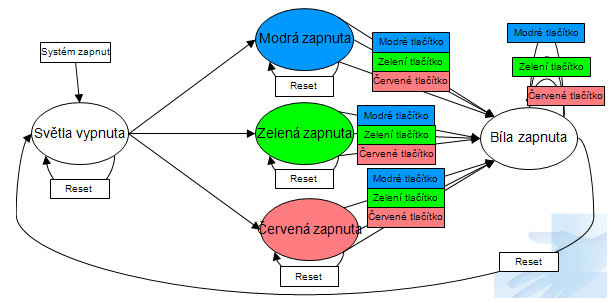
\includegraphics{test}   
\subsection{White-box}
vyžaduje znalost vnitřních datových a programových struktur a také toho, jak je systém naimplementován. Testerovi jsou v případě white box testování poskytnuty veškeré informace, to znamená, že má k dispozici nejen příslušnou dokumentaci, ale i binární a zdrojový kód testované aplikace. Tester musí zdrojovému kódu porozumět a analyzovat ho.
\subsubsection{Využití}
White box testování je velice vhodné např. pro webové služby a to obzvlášť na počátku vývojového cyklu, kdy vývojář a tester mohou spolupracovat na odhalování chyb. White box test můžeme využít ke zjištění, jak se systém chrání před neautorizovaným přístupem, jak je řízen přístup k jednotlivým částem aplikace a k datům, jak je implementována integritní ochrana nebo jak jsou ukládána hesla. White box test můžeme také použít k nalezení nežádoucího kódu, bezpečnostních chyb a zranitelností.
\subsubsection{metody testování}
\begin{itemize}
    \item Testování výrazů/instrukcí (Statement Testing)
    \item Testování skoků/rozhodování
    \item Testování toku dat
    \item Testování podmínek skoků
    \item Testování kombinace podmínek skoků
    \item Testování změny podmínky
\end{itemize}
\subsubsection{Testování výrazů/instrukcí}
Provede se každý výraz/instrukce kódu alespoň jednou během provádění testovacích případů
\subsubsection{Testování skoků/rozhodování}
Vytvoří se testovací případy tak aby se každé rozhodnutí provedlo s výsledkem TRUE a FALSE.
\subsection{Grey box}
Grey box testování předpokládá omezenou znalost interních datových a programových struktur za účelem navrhnutí vhodných testovacích scénářů, které se realizují na úrovni black box.
Způsob testování je tak kombinací black box a white box testování. Nejedná se o black box, protože tester zná některé vnitřní struktury, ale zároveň se nejedná ani o white box, protože znalosti vnitřních struktur nejdou do hloubky. Koncept grey box testování je velice jednoduchý. Jestliže tester ví, jak produkt funguje uvnitř, potom ho může lépe otestovat zvenku. Gray box test, stejně jako black box test je tedy prováděn zvenku, ale tester je lépe informován, jak jednotlivé komponenty fungují a spolupracují.
\subsubsection{Využití}
Typickým příkladem je, že white box test je použit k nalezení zranitelností a black box test je následně použit ke zjištění, zda je tyto zranitelnosti možné použít k úspěšnému provedení útoku. Se znalostí vnitřních struktur může tester lépe sestavit testovací scénáře, určit hranice hodnot atd. Grey box testu se obzvlášť používá, když se provádí integrační testování dvou modulů od dvou různých dodavatelů a je potřeba otestovat interfacy. Další velice častý případ užití je v případě testování vícevrstvé aplikace, kdy máme kontrolu nad vstupem, výstupem a máme přímý přístup do databáze. Můžeme tak porovnávat všechny tři hodnoty: vstup, hodnotu v databázi a výstup. Tímto způsobem můžeme zjistit, kde dochází k manipulaci s výsledkem, zda na straně klienta, aplikace nebo při zápisu či čtení z databáze nebo přímo v databázi například triggerem, který spustí nějakou uloženou proceduru. Dále můžeme prohlížet vytvořený HTML formulář, analyzovat skripty a práci s cookie. Stejně tak je možné použít tohoto přístupu k penetračnímu testování webové aplikace. Grey box testů se také s oblibou používá v okamžiku, kdy nechceme poskytnout zdrojové ani binární kódy, a zároveň nechceme, aby tester ztrácel čas skenováním sítě a inventarizací. V takovém případě mu informace o topologii sítě a architektuře aplikace poskytneme.
\subsubsection{Výhody}
\begin{itemize}
    \item Neúplné otestování – to je dáno tím, že binární ani zdrojové kódy nejsou k dispozici a není tak možné otestovat všechny datové toky.  Míra pokrytí těchto toků závisí hodně na schopnostech, znalostech a zkušenostech testera.
    \item Kvalita kódu – stejně jako u black box testu, to že něco funguje podle specifikace a je to odolné proti známým zranitelnostem, neznamená, že kód je efektivní a že aplikace neobsahuje žádný nežádoucí kód.

\end{itemize}
\subsubsection{Výhody}
\begin{itemize}
    \item Slučuje v sobě výhody black box i white box přístupu.
    \item Neintrusivní – přístup ke zdrojovému ani binárnímu kódu není třeba. Je založeno na znalosti funkční specifikace, rozhraní a architektuře aplikace.
    \item nteligentní testy – tester je schopen díky znalostem, byť omezeným, napsat inteligentní testovací scénáře zaměřené i na manipulaci s daty a použité komunikační protokoly.
\end{itemize}
\subsection{Distribuce pro testování bezpečnosti}
Existuje také řada operačních systémů zaměřených
na bezpečnostní testování. Typickým příkladem jsou různé distribuce Linuxu, které obsahují
širokou škálu ověřených nástrojů různých vývojářů, vyvinutých třeba i pro jeden účel.
\begin{itemize}
    \item Kali \url{http://www.kali.org}
    \item BackBox \url{http://www.backbox.org}
    \item Blackbuntu \url{http://www.blackbuntu.com}
    \item Pentoo \url{http://pentoo.ch}
    \item CAINE \url{http://www.caine-live.net}
    \item Fedora Security Lab \url{https://spins.fedoraproject.org/cs/security}
    \item Mariux \url{http://www.matriux.com}
    \item NodeZero \url{http://www.nodezero-linux.org}
    \item WEAKERTH4N \url{http://weaknetlabs.com}
\end{itemize}
\subsection{Nástroje na vyhledávání zranitelností}
\begin{itemize}
    \item Nessus \url{http://www.tenable.com}
    \item Nexpose \url{http://www.rapid7.com/products/nexpose}
    \item OpenVAS \url{http://www.openvas.org}
    \item Retina \url{http://go.beyondtrust.com/}
    \item Core Impact Pro \url{http://www.coresecurity.com/)}
    \item GFI LanGuard  \url{http://www.gfi.com/}
    \item Unified Security Management \url{https://www.alienvault.com/)}
    \item Tripwire SecureScan  \url{http://www.tripwire.com/}
\end{itemize}
\subsection{Nástroje specializované na zneužívání zranitelností}
\begin{itemize}
    \item Metasploit \url{http://www.metasploit.com}
    \item Core Impact Pro  \url{http://www.coresecurity.com/}
    \item Immunity CANVAS  \url{http://www.immunityinc.com/}
\end{itemize}
\subsection{ostatní}
\begin{itemize}
    \item OSWA-Assistant (http://securitystartshere.org/) – testování bezdrátových
sítí
\item CISOfy Lynis (https://cisofy.com/lynis/) – nástroj pro lokální testování zabezpečení
systémů založených na UNIXu. Vyskytuje se i v Kali Linux
\item Microsoft Baseline Security Analyzer (http://www.microsoft.com/) – kontroluje
zabezpečení, aktualizace a doporučená nastavení produktů společnosti Microsoft.
\end{itemize}

\end{document}